\documentclass[11pt,a4paper]{article}
\usepackage[margin=24mm]{geometry}\usepackage[T1]{fontenc}\usepackage[utf8]{inputenc}\usepackage{lmodern}\usepackage{microtype}
\usepackage{amsmath,amssymb,bm}\usepackage{booktabs,tabularx,longtable,array}\usepackage{graphicx,float,placeins}
\usepackage[dvipsnames]{xcolor}\usepackage{tikz}\usetikzlibrary{arrows.meta,positioning}\usepackage{hyperref}\usepackage{enumitem}\usepackage{fancyhdr}\usepackage[numbers]{natbib}
\definecolor{reportblue}{HTML}{174A7E}\definecolor{reportgreen}{HTML}{2E7D32}\definecolor{reportorange}{HTML}{C76B00}
\hypersetup{colorlinks=true,linkcolor=reportblue,citecolor=reportblue,urlcolor=reportblue}
\setlength{\parindent}{0pt}\setlength{\parskip}{.55em}
\pagestyle{fancy}\fancyhf{}\lhead{Structured $SO(3)$ Latents}\rhead{18 September 2026}\cfoot{\thepage}
\newcommand{\SO}{\mathrm{SO}}\newcommand{\so}{\mathfrak{so}}\newcommand{\R}{\mathbb R}\newcommand{\vct}[1]{\bm{#1}}
\newenvironment{keyresult}{\begin{quote}\color{reportgreen}\textbf{Key result.} }{\end{quote}}
\newenvironment{caution}{\begin{quote}\color{reportorange}\textbf{Important qualification.} }{\end{quote}}
\begin{document}
\begin{titlepage}\centering\vspace*{24mm}
{\Huge\bfseries\color{reportblue} Ball World Model\par}\vspace{5mm}
{\LARGE Structured $SO(3)$ Context Latents, $\so(3)$ Motion Latents, and Intrinsic Evaluation\par}\vspace{15mm}
\fbox{\parbox{.84\textwidth}{\centering\large RGB sequence $\rightarrow$ group-valued configuration, Lie-algebra motion, equivariant carriers, scalar features, and artifacts}}
\vfill{\Large Dr. Jasper Juchem\par}\vspace{4mm}
{\large Stand-alone technical report for machine-learning and dynamical-systems researchers\par}\vspace{10mm}
{\large Evaluation dated 18 September 2026\par}{\large Revised intrinsic-evaluation edition\par}
\end{titlepage}

\begin{abstract}
This report evaluates a rotation-only visual observer whose latent representation explicitly contains an $SO(3)$ configuration sector and an $\so(3)$ motion sector. Unlike the preceding model, rotational evolution is no longer represented by an additive Euler step in an unconstrained Euclidean content latent. The model predicts a group element $G_t$ and generator $\xi_t$, then evolves the latent intrinsically through $\hat G_{t+1}=\exp(\!\Delta t[\xi_t]_\times)G_t$. A $K=24$ equivariant carrier gives the geometric sector high ambient capacity, while scalar and artifact sectors retain non-manifold visual information. Decoded-state refinement is disabled, so the experiment isolates latent geometry.

The observer preserves excellent state estimation: mean orientation error is $0.386^\circ$, with $0.864^\circ$ at the 95th percentile, while angular-velocity $R^2$ remains above 0.9948 on all axes. The new intrinsic diagnostics make the story substantially clearer. Encoded rotations satisfy orthogonality and unit determinant to approximately $10^{-7}$. The learned one-step group transition has mean residual $0.01247$ rad=$0.714^\circ$, and forward/backward increments have mean inverse residual $0.001775$ rad=$0.102^\circ$. Recursive intrinsic rollout grows gradually from $0.730^\circ$ mean error at one interval to $2.363^\circ$ at nine intervals.

Sector-wise metrics also reveal a limitation. The canonical three-dimensional generator is nearly perfectly aligned with physical angular velocity, but the 141-dimensional motion-artifact sector also predicts angular velocity with mean $R^2\approx0.997$. Thus the geometric sector works and is sufficient, but the motion representation is not disentangled: physical motion is redundantly copied into artifacts. The added evaluation therefore strengthens the claim that valid and operational group geometry exists in the latent, while simultaneously weakening any claim of clean sector separation or proven generalization.
\end{abstract}
\tableofcontents\clearpage

\section{Scope and scientific question}
The experiment asks whether rotational structure can be moved from a case-specific decoder and world-coordinate corrector into the learned representation itself. The evaluated configuration uses 24 geometric carrier channels, 16 scalar coordinates, 256-dimensional context and motion representations, and zero refinement iterations. The empirical source contains 1,050 test windows, 10,500 frame orientations, and 9,450 adjacent intervals.

The relevant distinction is between three claims:
\begin{enumerate}[leftmargin=*]
\item \textbf{Type validity}: the designated context variable is numerically an element of $SO(3)$.
\item \textbf{Operational geometry}: the learned generator produces accurate group transitions, inverses, and finite-horizon compositions.
\item \textbf{Representational separation and generalization}: the designated sectors uniquely carry physical information and improve robustness outside the training distribution.
\end{enumerate}
The new evaluation strongly addresses the first two claims. It exposes unresolved issues for the third.

\section{Structured latent strategy}
\begin{figure}[H]\centering\resizebox{\textwidth}{!}{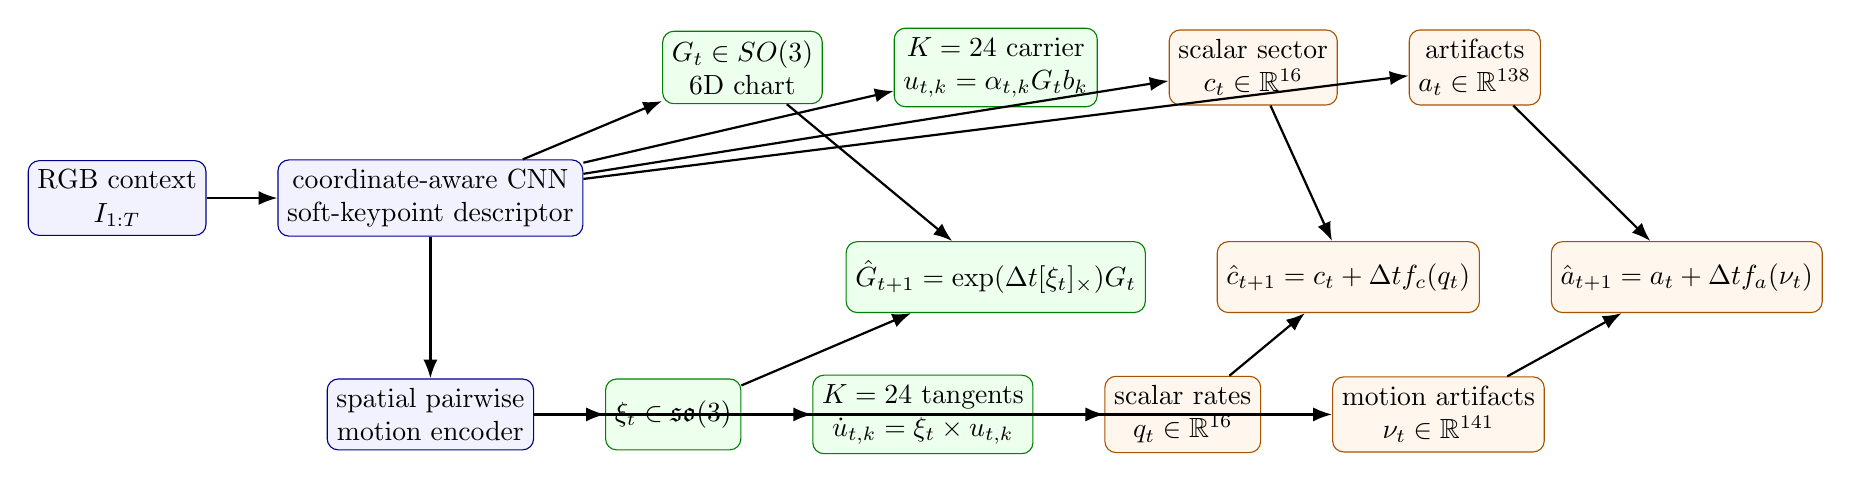
\begin{tikzpicture}[node distance=8mm and 9mm,
box/.style={draw=blue!55!black,fill=blue!5,rounded corners,align=center,minimum height=9mm},
geo/.style={draw=green!50!black,fill=green!7,rounded corners,align=center,minimum height=9mm},
aux/.style={draw=orange!65!black,fill=orange!7,rounded corners,align=center,minimum height=9mm},
arr/.style={-{Latex[length=2.4mm]},thick}]
\node[box] (rgb) {RGB context\\$I_{1:T}$};
\node[box,right=of rgb] (enc) {coordinate-aware CNN\\soft-keypoint descriptor};
\node[geo,above right=7mm and 10mm of enc] (G) {$G_t\in SO(3)$\\6D chart};
\node[geo,right=of G] (U) {$K=24$ carrier\\$u_{t,k}=\alpha_{t,k}G_tb_k$};
\node[aux,right=of U] (c) {scalar sector\\$c_t\in\mathbb R^{16}$};
\node[aux,right=of c] (a) {artifacts\\$a_t\in\mathbb R^{138}$};
\node[box,below=18mm of enc] (me) {spatial pairwise\\motion encoder};
\node[geo,right=of me] (w) {$\xi_t\in\mathfrak{so}(3)$};
\node[geo,right=of w] (T) {$K=24$ tangents\\$\dot u_{t,k}=\xi_t\times u_{t,k}$};
\node[aux,right=of T] (q) {scalar rates\\$q_t\in\mathbb R^{16}$};
\node[aux,right=of q] (n) {motion artifacts\\$\nu_t\in\mathbb R^{141}$};
\node[geo,below=17mm of U] (step) {$\hat G_{t+1}=\exp(\Delta t[\xi_t]_\times)G_t$};
\node[aux,right=of step] (sstep) {$\hat c_{t+1}=c_t+\Delta t f_c(q_t)$};
\node[aux,right=of sstep] (astep) {$\hat a_{t+1}=a_t+\Delta t f_a(\nu_t)$};
\draw[arr](rgb)--(enc);\draw[arr](enc)--(G);\draw[arr](enc)--(U);\draw[arr](enc)--(c);\draw[arr](enc)--(a);\draw[arr](enc)--(me);
\draw[arr](me)--(w);\draw[arr](me)--(T);\draw[arr](me)--(q);\draw[arr](me)--(n);\draw[arr](G)--(step);\draw[arr](w)--(step);\draw[arr](c)--(sstep);\draw[arr](q)--(sstep);\draw[arr](a)--(astep);\draw[arr](n)--(astep);
\end{tikzpicture}
}\caption{Structured context and motion latents. Green sectors carry prescribed group actions; orange sectors retain scalar or unrestricted visual information.}\end{figure}

\subsection{Context latent}
The packed context representation is
\begin{equation}
z_t^c=(r_t^{6D},\alpha_t,U_t,c_t,a_t)\in\R^{256},
\end{equation}
where $r_t^{6D}$ constructs $G_t\in SO(3)$ through a continuous 6D map \citep{zhou2019rotation6d},
\begin{equation}
u_{t,k}=\alpha_{t,k}G_tb_k,\qquad k=1,\ldots,24,
\end{equation}
$c_t\in\R^{16}$ is scalar under the group action, and $a_t\in\R^{138}$ is unrestricted. The 72 carrier coordinates form 24 copies of the standard vector representation. Their ambient rank can exceed the intrinsic group dimension without changing the three-dimensional nature of the group orbit.

\subsection{Motion latent}
The motion representation is
\begin{equation}
z_t^m=(\xi_t,\dot\alpha_t,\dot U_t,q_t,\nu_t)\in\R^{256},
\end{equation}
with $\xi_t\in\so(3)\simeq\R^3$ and
\begin{equation}
\dot u_{t,k}^{\rm geom}=\xi_t\times u_{t,k}.
\end{equation}
The motion scalar sector $q_t\in\R^{16}$ can describe coordinate-free confidence, visibility, or speed magnitude. The motion artifact sector $\nu_t\in\R^{141}$ is intended for residual visual change not assigned to the physical tangent structure.

\subsection{Intrinsic transition}
The rotational context state evolves by
\begin{equation}
\hat G_{t+1}=\exp(\Delta t[\xi_t]_\times)G_t.
\end{equation}
Scalar and artifact sectors use learned residual prediction,
\begin{equation}
\hat c_{t+1}=c_t+\Delta t f_c(q_t),\qquad
\hat a_{t+1}=a_t+\Delta t f_a(\nu_t).
\end{equation}
This separates geometric evolution from observation-specific dynamics. The current model remains an observer because $\xi_t$ is inferred from both endpoint images.

\section{Training and evaluation design}
Ground-truth orientation and angular velocity provide a geometry-preserving teacher:
\begin{equation}
R_t^{gt}\mapsto \{R_t^{gt}b_k\}_{k=1}^{24},\qquad
\omega_t^{gt}\mapsto\{\omega_t^{gt}\times R_t^{gt}b_k\}_{k=1}^{24}.
\end{equation}
The objective combines geodesic orientation alignment, normalized generator alignment, carrier and tangent alignment, forward/backward group prediction, reversal consistency, amplitude anchoring, and predictive learning for scalar and artifact sectors. Stopped-target latent prediction resembles the broad joint-embedding strategy \citep{assran2023ijepa}.

The normal evaluation reports state accuracy, temporal interventions, packed-latent probes, and effective rank. The structured extension additionally reports group validity, one-step group consistency, inverse consistency, recursive rollout, sector-wise ranks, and sector-wise angular-velocity probes.

\section{State estimation results}
\subsection{Orientation}
\begin{keyresult}
Mean orientation error is $0.3861^\circ$, median error is $0.3217^\circ$, and the 95th percentile is $0.8639^\circ$. The maximum is $2.9009^\circ$. All are achieved without decoded-state refinement.
\end{keyresult}

\begin{figure}[H]\centering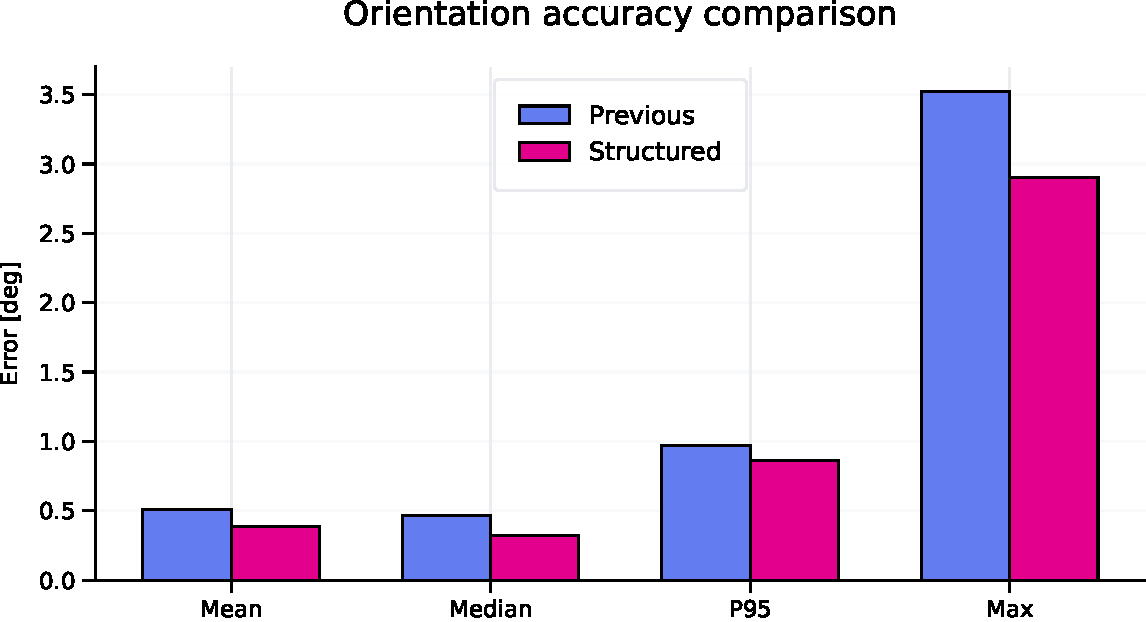
\includegraphics[width=.72\textwidth]{figures/orientation_comparison.pdf}\caption{The structured model improves orientation error relative to the preceding rotation observer.}\end{figure}

Compared with the earlier observer, mean error improves by 23.8\%, median by 31.2\%, P95 by 11.0\%, and maximum by 17.7\%. This is strong evidence of structural non-inferiority and a favorable orientation trend, though not yet a controlled multi-seed architecture comparison.

\subsection{Angular velocity}
Component RMSE is $0.575$, $1.240$, and $0.646$ rad/s for $x,y,z$, with $R^2=0.99897,0.99484,0.99864$. Pointwise angular-velocity error is somewhat worse than the previous observer, especially in $y$, while remaining excellent relative to the approximately 29.3 rad/s mean speed.

\begin{figure}[H]\centering
\includegraphics[width=.92\textwidth]{figures/angular_velocity_component_scatter.png}\caption{Predicted versus true angular velocity.}\end{figure}

\subsection{Temporal interventions}
Reversing the input preserves mean speed and reverses direction with a residual of $1.107$ rad/s. Repeating one frame reduces mean inferred speed from 29.315 to 0.067 rad/s, a 99.77\% reduction. Shuffling changes the generator strongly. These results show that the Lie-algebra coordinate depends on directed temporal evidence rather than static orientation.

\section{Intrinsic group validity}
\begin{table}[H]\centering\caption{Validity and intrinsic consistency of the structured latent.}\begin{tabular}{lrrrr}\toprule
Metric & Mean & Median & P95 & Maximum\\\midrule
Orthogonality, Frobenius & $1.55\times10^{-7}$ & $1.49\times10^{-7}$ & $2.94\times10^{-7}$ & $4.98\times10^{-7}$\\
Determinant residual & $9.11\times10^{-8}$ & $1.19\times10^{-7}$ & $2.38\times10^{-7}$ & $4.17\times10^{-7}$\\
One-step residual [rad] & 0.01247 & 0.00979 & 0.02907 & 0.42707\\
Inverse residual [rad] & 0.001775 & 0.001381 & 0.003997 & 0.02121\\\bottomrule
\end{tabular}\end{table}

\begin{figure}[H]\centering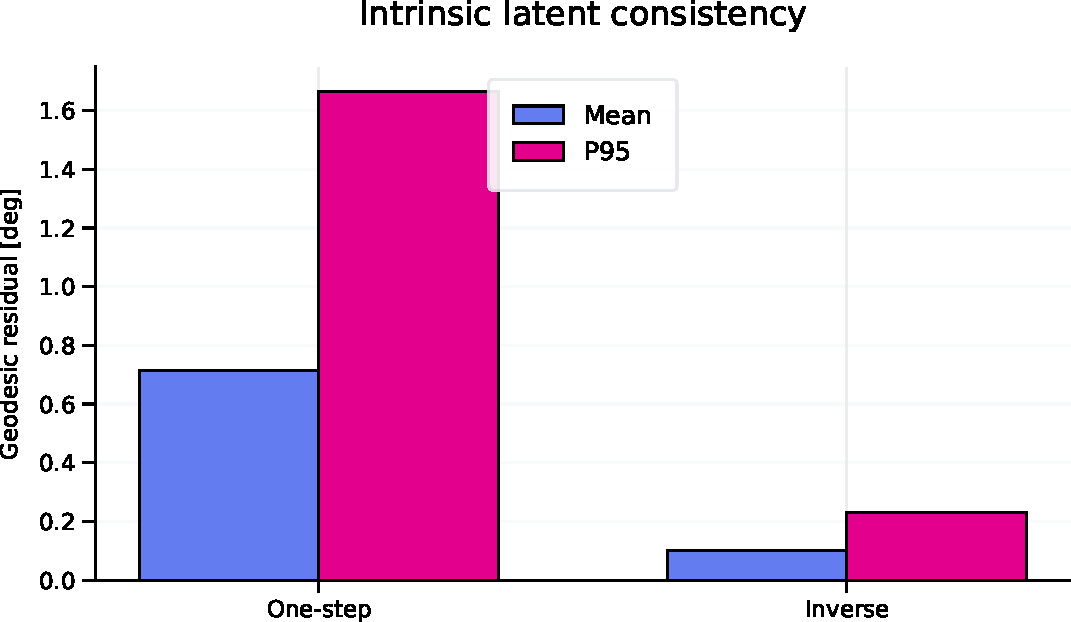
\includegraphics[width=.7\textwidth]{figures/group_consistency.pdf}\caption{Intrinsic latent one-step and inverse residuals.}\end{figure}

The orthogonality and determinant results prove numerical membership in $SO(3)$ to floating-point precision. This is primarily a construction check because the 6D projection enforces group validity. More scientifically informative are the transition results: the mean one-step residual is $0.714^\circ$, with P95 $1.665^\circ$, and the mean inverse residual is only $0.102^\circ$, with P95 $0.229^\circ$.

\begin{caution}
The one-step group residual is larger than the direct orientation error of $0.386^\circ$. This means the separately encoded endpoint orientations are more accurate than the endpoint obtained by advancing the inferred generator for one interval. The group operation is valid, but generator noise still limits transition accuracy.
\end{caution}

\section{Intrinsic rollout}
\begin{figure}[H]\centering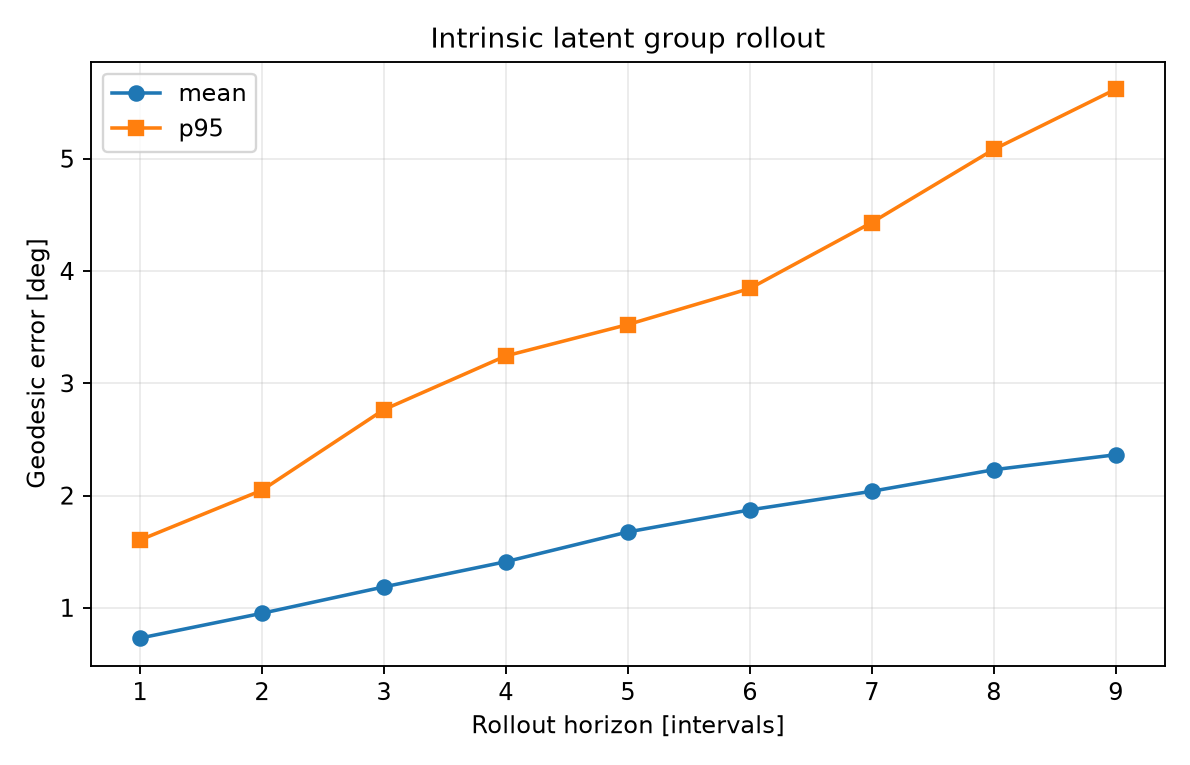
\includegraphics[width=.78\textwidth]{figures/rollout_by_horizon.png}\caption{Recursive group rollout using inferred interval generators.}\end{figure}

\begin{table}[H]\centering\caption{Selected intrinsic rollout horizons.}\begin{tabular}{rrrr}\toprule
Intervals & Mean [deg] & Median [deg] & P95 [deg]\\\midrule
1 & 0.730 & 0.588 & 1.604\\
3 & 1.186 & 0.926 & 2.765\\
5 & 1.675 & 1.227 & 3.523\\
7 & 2.038 & 1.481 & 4.432\\
9 & 2.363 & 1.693 & 5.619\\\bottomrule
\end{tabular}\end{table}

The recursive error increases smoothly rather than catastrophically. Over nine 10 ms intervals, mean error reaches $2.36^\circ$. This is evidence that the algebra coordinate composes coherently over the observed context. It is not an autonomous rollout because each interval generator is inferred from observed endpoint frames. A true open-loop test would infer one initial generator or predict future generators without future images.

\section{Sector-wise structure}
\subsection{Effective dimension}
\begin{figure}[H]\centering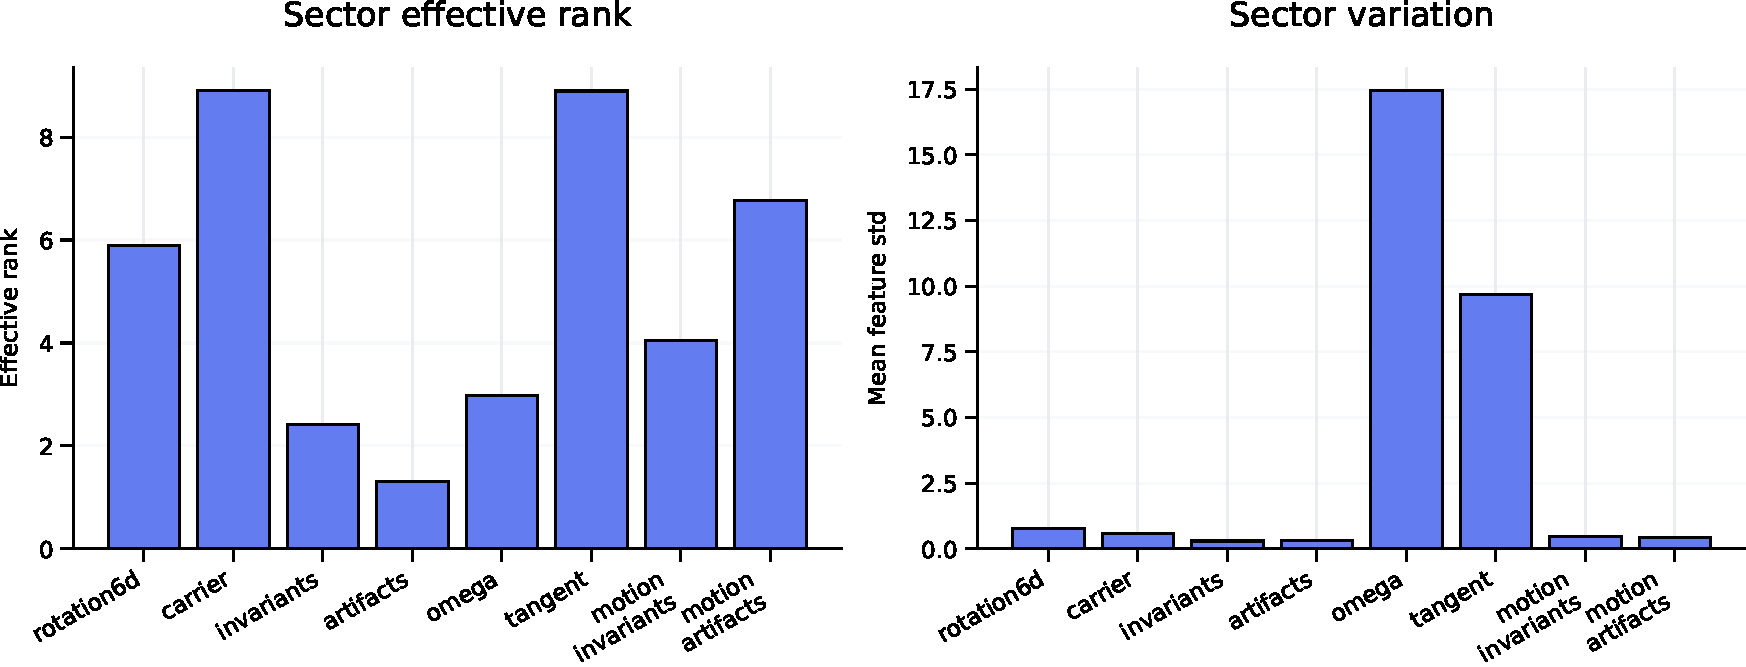
\includegraphics[width=.96\textwidth]{figures/sector_statistics.pdf}\caption{Sector-wise rank and variation.}\end{figure}

\begin{table}[H]\centering\caption{Sector statistics.}\begin{tabular}{lrrr}\toprule
Sector & Dimension & Mean feature std & Effective rank\\\midrule
Rotation 6D & 6 & 0.783 & 5.887\\
Carrier & 72 & 0.579 & 8.909\\
Context invariants & 16 & 0.301 & 2.409\\
Context artifacts & 138 & 0.316 & 1.305\\
Canonical $\omega$ & 3 & 17.461 & 2.980\\
Tangent carrier & 72 & 9.672 & 8.896\\
Motion invariants & 16 & 0.475 & 4.053\\
Motion artifacts & 141 & 0.426 & 6.770\\\bottomrule
\end{tabular}\end{table}

The carrier and tangent sectors use substantially more effective dimensions than their canonical variables, supporting the motivation for a rich representation. The context artifact sector is nearly rank one, suggesting that 138 artifact dimensions are largely unused in this controlled fixed-rendering experiment. This is not necessarily harmful, but indicates over-allocation of context artifact capacity for the present data.

\subsection{Angular-velocity sufficiency and leakage}
\begin{figure}[H]\centering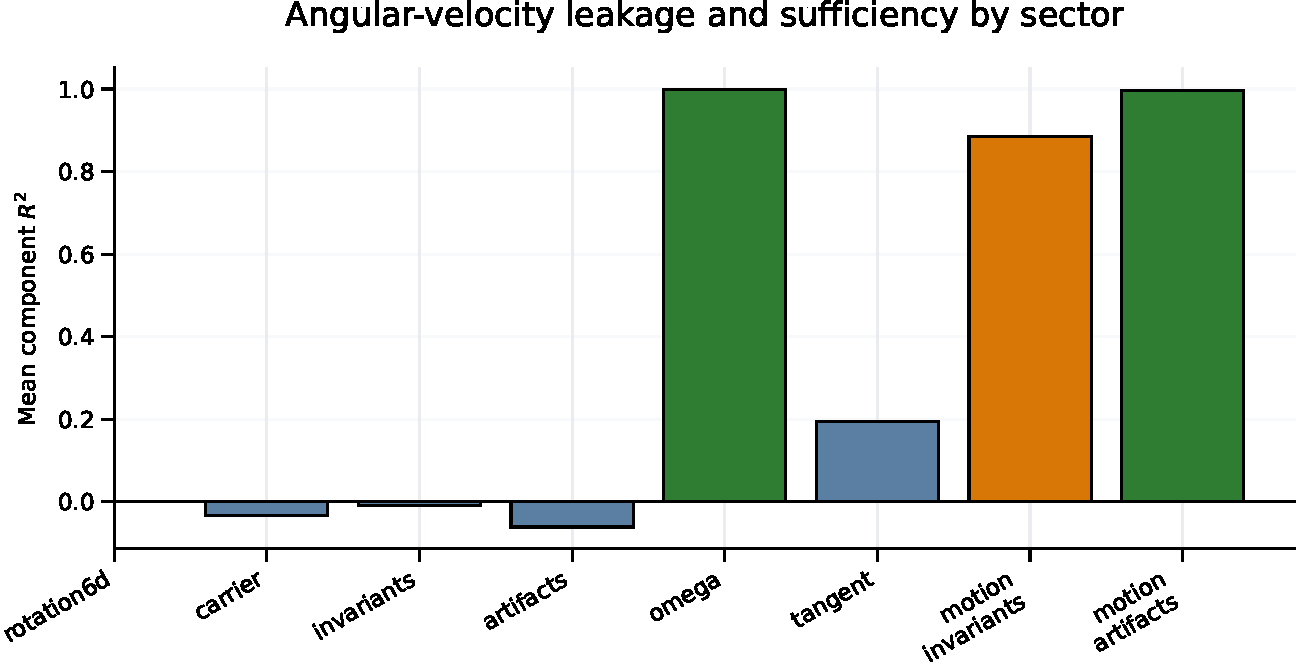
\includegraphics[width=.86\textwidth]{figures/sector_omega_probe.pdf}\caption{Mean component $R^2$ for angular velocity decoded from individual sectors.}\end{figure}

The canonical generator performs as intended: a linear probe obtains $R^2=0.99966,0.99901,0.99969$ for $x,y,z$. Context carriers, context invariants, and context artifacts contain essentially no signed angular-velocity information, which supports content-motion separation.

The motion result is more nuanced. Tangent vectors alone have modest linear $R^2$ between 0.154 and 0.248. This is expected because $\dot u=\omega\times u$ is bilinear in orientation and angular velocity; recovering $\omega$ from tangents alone requires the base carrier or a nonlinear operation. By contrast, motion invariants have substantial angular-velocity information, with $R^2$ from 0.797 to 0.951.

Most importantly, motion artifacts yield $R^2=0.99751,0.99592,0.99733$. The artifact branch therefore redundantly contains nearly the full physical angular velocity.

\begin{caution}
The new results establish a valid and accurate geometric sector, but they do not establish disentanglement. The motion artifact sector can almost reproduce $\omega$. This does not compromise the canonical generator's correctness, because physical output and group transition use $\xi_t$. It does weaken claims that non-geometric sectors contain only irrelevant visual artifacts or that a future module can discard them without losing all dynamically useful information.
\end{caution}

\section{Does the new evaluation make the story more convincing?}
Yes, but in a more precise and balanced way.

\paragraph{The story is more convincing because:}
\begin{enumerate}[leftmargin=*]
\item The group sector is numerically valid to $10^{-7}$.
\item The learned generator advances the group with a measured one-step residual rather than merely producing a good decoded output.
\item Forward and backward increments are close to inverses.
\item Intrinsic composition remains stable over nine intervals.
\item Canonical $\omega$ is almost perfectly linearly aligned with physical angular velocity.
\item The $K=24$ carrier and tangent sectors have nontrivial effective rank near 8.9, validating the richer-than-state representation idea.
\item Context artifacts do not encode signed angular velocity, and repeated frames drive the generator almost exactly to zero.
\end{enumerate}

\paragraph{The story is not yet a generalization result because:}
\begin{enumerate}[leftmargin=*]
\item Group validity is partly guaranteed by construction.
\item Rollout uses interval generators inferred using future endpoint observations.
\item No held-out frame rate, speed band, orientation region, camera, or appearance test is included.
\item No dimension-matched Euclidean ablation has been evaluated with identical seeds.
\item The motion-artifact sector heavily duplicates physical angular velocity.
\end{enumerate}

The corrected conclusion is therefore:

\begin{keyresult}
The model has learned an operational $SO(3)/\so(3)$ latent interface whose group action is valid, whose inverse relation is accurate, and whose finite-horizon composition is stable. This goes substantially beyond showing that a decoder can output a rotation matrix. However, the current representation is redundantly entangled, and improved out-of-distribution generalization remains a hypothesis rather than an established result.
\end{keyresult}

\section{Recommended next experiments}
\subsection{Joint tangent decoding}
The current tangent-only probe is structurally unfair. Recover $\omega$ from the pair $(U,\dot U)$, not $\dot U$ alone. The analytic least-squares relation for unit carriers is
\begin{equation}
\hat\omega=\left(\sum_k(\|u_k\|^2I-u_ku_k^T)\right)^{-1}\sum_k u_k\times\dot u_k.
\end{equation}
This should verify that the tangent carrier encodes the generator when paired with its base point.

\subsection{Artifact bypass tests}
Zero the motion artifact sector and confirm that state output and group rollout are unchanged. Then train a model with artifact-sector gradient reversal or an information bottleneck against signed $\omega$. Compare whether rollout or appearance prediction suffers.

\subsection{True open-loop rollout}
Infer a context-level generator and propagate it without future images. Constant-$\omega$ data make this test especially clean:
\begin{equation}
\hat G_{t+h}=\exp(h\Delta t[\hat\omega]_\times)G_t.
\end{equation}
Compare against the Euclidean baseline over horizons longer than the ten-frame context.

\subsection{Distribution shifts}
Train and test on disjoint angular-speed shells, held-out regions of $SO(3)$, new frame strides, and changed marker or lighting conditions. These tests target the proposed value of latent geometry directly.

\subsection{Controlled ablation}
Train at least three seeds of: the previous Euclidean latent; the structured model; and a dimension-matched Euclidean partition using the same losses where possible. Report confidence intervals for state error, intrinsic rollout, and intervention residuals.

\section{Conclusion}
The structured evaluation materially improves the scientific story. It confirms that $SO(3)$ is not merely imposed after decoding: the designated context variable is a valid group element, the designated motion variable generates intrinsic transitions, forward and backward increments nearly invert one another, and recursive composition is stable across the observed horizon. The $K=24$ carrier provides higher-dimensional geometric structure with effective rank near nine, showing that geometric representation need not collapse to the minimal physical state dimension.

At the same time, the new diagnostics prevent an overstatement. The motion artifact sector contains almost all angular-velocity information, so the present model implements a correct structured pathway but not a cleanly separated one. The next phase should therefore focus less on another aggregate RMSE improvement and more on causal sector ablations, joint carrier-tangent decoding, true open-loop rollout, and distribution-shift tests. Those experiments will determine whether the latent geometry merely coexists with accurate perception or provides the intended gains in modularity and generalization.

\appendix
\section{Key numerical values}
\begin{itemize}[leftmargin=*]
\item Orientation mean/median/P95/maximum: 0.3861/0.3217/0.8639/2.9009 degrees.
\item Group orthogonality and determinant mean residuals: $1.55\times10^{-7}$ and $9.11\times10^{-8}$.
\item One-step latent group residual: mean 0.714 degrees, P95 1.665 degrees.
\item Forward-backward inverse residual: mean 0.102 degrees, P95 0.229 degrees.
\item Nine-interval rollout: mean 2.363 degrees, P95 5.619 degrees.
\item Canonical $\omega$ probe mean $R^2$: approximately 0.99945.
\item Motion-artifact probe mean $R^2$: approximately 0.99692.
\item Carrier and tangent effective ranks: 8.909 and 8.896.
\end{itemize}

\bibliographystyle{plainnat}\bibliography{references}
\end{document}
